\chapter{Programming Embedded Systems}

\section{Introduction}
\adef{Embedded system} is a system in which the computer (generally a microcontroller or microprocessor) is included as an integral part of the system.
\textbf{Constraints}
\begin{itemize}
    \item Timing 
    \item Cost 
    \item Weight 
    \item Power 
    \item Memory
    \item Computation power
\end{itemize}

\adef{SDK} stands for software development kit and it provides an interface to abstract the specific hardware.

A clear and precise description of the problem that a function solves is called a \textit{contract} for the function.
\url{http://www.cs.ecu.edu/karl/2310/Javanotes/contract1.html}

\textit{Frama-C} is an open-source extensible and collaborative platform dedicated to source-code analysis of C software. The Frama-C analyzers assist you in various source-code-related activities, from the navigation through unfamiliar projects up to the certification of critical software. 
\url{https://frama-c.com/}

\textit{Zephyr} is a small real-time operating system (RTOS)[6] for connected, resource-constrained and embedded devices (with an emphasis on microcontrollers) supporting multiple architectures and released under the Apache License 2.0.
\url{https://en.wikipedia.org/wiki/Zephyr_(operating_system)}


\section{From Hardware to operating system}
This section describes the terminology and what is needed to run 
a full operating system like debian.


\subsection{Hardware}
The main component of the hardware is the microcontroller.
ARM Cortex is a popular family CPU architecture.
These include a three CPU architecture profiles: A-profile (Application);
R-profile (Real-Time); M-profile (Microcontroller);
Some popular manufactures are STMicroelectronics and Microchip.
The microcontroller is soldered on to a PCB, which has the required 
electronic components, peripherals, and connectors.
%https://www.arm.com/architecture/cpu?utm_source=google&utm_medium=cpc&utm_content=text_txt_na_cpu&utm_campaign=mk30_brand-paid_architecture_2023_awareness_keyword_na&utm_term=arm%20cpu%20architecture&gad_source=1&gclid=CjwKCAiAloavBhBOEiwAbtAJO1rUN-gGmSbR6WJQtGEBNwXjmRD4gjYYc7Or6Ciu3wYLcLp-dot9WxoC-IUQAvD_BwE


\subsection{Firmware}
Firmware is software embedded on the hardware, e.g., ROM, and is responsible 
for initializing device drivers and configuration. BIOS is part of the firmware 
and let the user low-level control for hardware devices.

It is also responsible to load the boot loader into memory during 
the handoff procedure.

% TODO: what firmware is available


\subsection{Boot loader}
The boot loader is responsible to load the operating system with the kernel
into memory.

An example of loader is GRUB, which is common for linux.


\subsection{Kernel and Operating System}
The kernel is a part of the operating system. It is responsible for 
manages system resources, such as memory, processes, and hardware devices

Linux is a popular kernel, especial for servers, but is also used 
in embedded system.

There are many linux distributions that runs the linux kernel.
A popular is debian, which raspberry pi OS is based on.

%drivers, peripherals


\section{States Machines}
\adef{Bare metal} is a system with a very simple application.
It doesn't have any specific timing requirements and is considered
to be a single loop application. Purely interrupt-based system.

\adef{RTOS} has multiple, independent execution threads. Usually
needs more memory and it is more elaborate data exchange between tasks.

\adef{State machines} A state machine shows the dynamic flow to states depending on values from previous states or user inputs.

When designing a state machines we need to first figure otu the 
states of the system. Then what are the state change triggers.
After that we want to define what happens when these triggers happens,
what is the next state.

\adef{State centric state machine} basically a big if-else statements 
that determine exactly what happens when we are in a state and how we get out.
The main issue with state centric state machine is that it becomes difficult to maintain. 
It is also continous computing, even if there is no update.
And using a get event function does not allow for debouncing.

\subsection{Debouncing}
A button press is not a clean input. If it is not handled each button press will be registered as several button presses.
There is a solution, however, \textit{Debouncing}.
\begin{itemize}
    \item Hardware debouncing: using a schmitt trigger.
    \item software debouncing: See figure \ref{fig:software_debouncing}. There is a delay between sensing an input, so if input comes each ms it will not count if the delay is 100ms.
\end{itemize}

\begin{figure}[H]
    \centering
    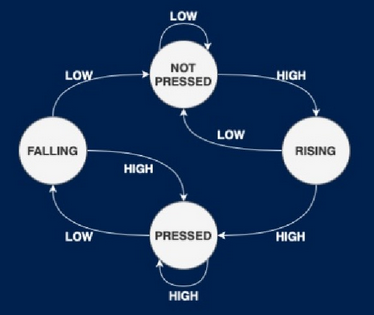
\includegraphics[width=10cm]{\imagesPath/software_debouncing.png}
    \caption{software debouncing}
    \label{fig:software_debouncing}
\end{figure}


\subsection{Hardware Interrupts}
Examples of interrupts
\begin{itemize}
    \item Clock interrupts
    \item Other internal interrupts: error like division by zero
    \item External interrupts: input from pins
\end{itemize}
All interrupts should be specified in the processor datasheet.

Interrupt service routine (ISR) is a software routine that the hardware invokes when there is a interrupt.
These interrupts can be stored in global/static variables or in a thread safe queue to handle 
them when there is time.

\adef{Deferred Interrupt Handling} is when the interrupt handler just record
the event and try to do as little as possible so that the priority of the task, 
which will react on the event, is the one who decides when to run.

\subsection{Table driven state machine}
Instead of state machine with a bunch of switch cases of if statements, it is possible to create a table
from the current state describes what happens when an event happens. This makes it easier to update and requires less code.
\begin{figure}[H]
    \centering
    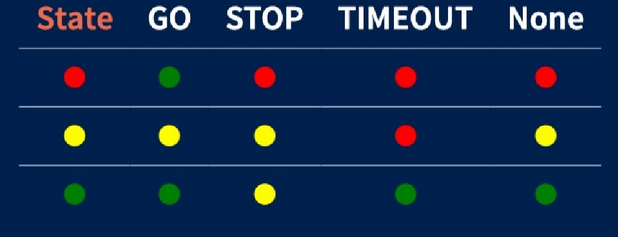
\includegraphics[width=10cm]{\imagesPath/table_driven_state_machine.png}
    \caption{Table driven state machine}
    \label{fig:table_driven_state_machine}
\end{figure}


\section{Zephyr}
The reason why we use realtime operating systems is that 
we want deterministic behavior and is particular important 
safety critical systems.

\begin{figure}[H]
    \centering
    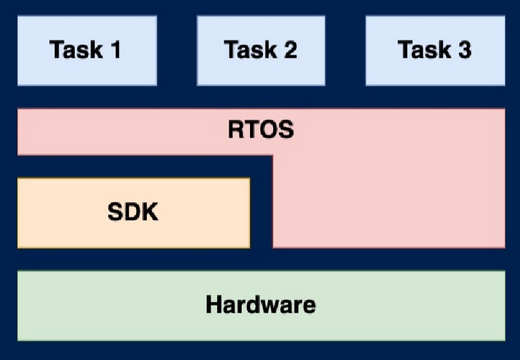
\includegraphics[width=10cm]{\imagesPath/zephyr_architecture.png}
    \caption{RTOS architecture}
    \label{fig:rtos_architecture}
\end{figure}

\subsection{Zephyr threads}
A thread is a kernel objects that is used when the application is to 
complex to be performed by an ISR
The number of threads that can be created is limited by RAM.

Spawning a thread statically:
\begin{verbatim}
    K_THREAD_DEFINE(thread_id, stack_size, 
        entry_point_function, arg1, arg2, arg3,
        priority, start_delay, execution_mode);
\end{verbatim}

\begin{figure}[H]
    \centering
    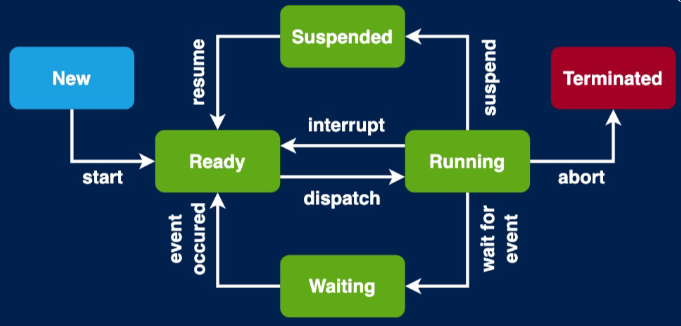
\includegraphics[width=10cm]{\imagesPath/thread_states.png}
    \caption{Thread states}
    \label{fig:thread_states}
\end{figure}

\begin{figure}[H]
    \centering
    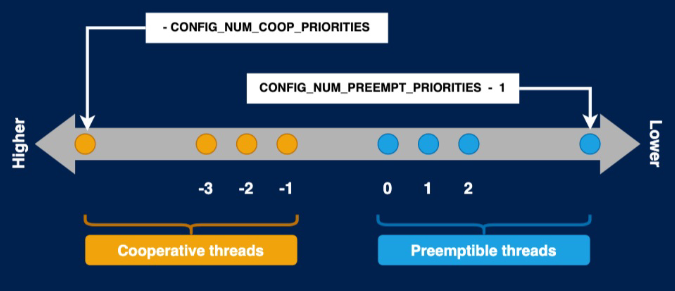
\includegraphics[width=10cm]{\imagesPath/thread_priorities.png}
    \caption{Thread priorities. Cooperative threads are non-preemptible, 
    when the highest priority task has been dispatched then it wont be preempted 
    even if a higher priority task is in the ready queue. Preempted threads 
    has a lower priority and are allowed to be preempted.}
    \label{fig:thread_priorities}
\end{figure}


\subsection{Communication}
Communication between threads can be ether shared memory (not stack since each thread has its own stack)
or message passing. 

\subsubsection{Shared memory and the use of locks}
Global and/or static variables needs to be carefully managed.
However, this is not a problem if we use cooperative threads, otherwise we have to use locks. 
Using locks can result in priority inversion (a higher priority task is preambled by a lower priority task) 
or deadly embrace (also known as deadlock).
Semaphores can also be used, they are more useful for sending signals.
Semaphores are taken/given unlike mutex which are locked/unlocked.

\subsubsection{Reentrant function}
Function which executes correctly even when called by more than one task.
It must follow certain rules:
\begin{itemize}
    \item Must not use any global variables that can change.
    \item Must not call non-reentrant functions.
    \item Must not use hardware in a non-atomic way.
\end{itemize}

\subsubsection{Message passing}
Message passing is more high-level way of communicating and is often considered.
The implementation is dependent on the RTOS.

\subsection{Zephyr architecture}
Code can be reused since the hardware is abstracted by having \textit{arch}, \textit{soc}, and \textit{board}.
If we want to create our own board, we can just add it in \textit{boards}.

\subsubsection{Device tree}
The OS should be able to run on different HW platforms, which is possible through the use of device tree.
A device tree represent the hardware configuration int o special data structure.
The HW layout is specified in a .dts file and can be extended with the use of .overlay file.
The .overlay file writes over the .dts file to get a more specific layout of the HW.
Linux compiles the .dts file into a binary representation used during boot-up. 
For zephyr it compiles into a header file.

\subsubsection{Other}
ISR should be as minimal as possible, it should use semaphore to unlock tasks which do the actual work.

\adef{Volatile}, whenever a variable is shared between two tasks, or a task and an ISR.
C qualifier volatile: We tell the compiler that it cannot relay on previously read values. 
C compilers usually do some optimization however if it is volatile it can not 
do so.

\section{Specification}
Types of requirements (FURPS+)
\begin{itemize}
    \item Functionality
    \begin{itemize}
        \item Features, capabilities, security
    \end{itemize}
    \item Usability
    \begin{itemize}
        \item Human-computer interaction
        \item Documentation
    \end{itemize}
    \item Reliability
    \begin{itemize}
        \item Frequency of failure
        \item Error recovery
    \end{itemize}
    \item Performance
    \begin{itemize}
        \item Response time 
    \end{itemize}
    \item Supportability
    \begin{itemize}
        \item Adaptability, Configurability
        \item Maintenance
    \end{itemize}
    \item Many others
    \begin{itemize}
        \item Adaptability
        \item User interface
        \item Licencing
    \end{itemize}
\end{itemize}

\adef{Function contracts} describes the intended behavior as a function between the \textit{caller} and the \textit{callee}.
It consists of a pair of a set of \textit{preconditions} (assumptions) and a set of preconditions (guarantees).

A formal specification is not expressed in nature language, but instead is formally specified with logic.

\adef{FOL properties} can be \textit{satisfiable}, \textit{valid}, \textit{ unsatisfiable}, \textit{invalid},
and can be solved with \textit{satisfiability modulo theories} (SMT) solver.

\adef{Assertion} an alternative to contracts to test if a preconditions or preconditions holds true.
However, there are som issues with assertions, they mixs specification and implementation, and mixes responsibilities of the caller and the callee.

\textit{Observers} is separate from the controller, it will check that the controller is behaving as expected.
\begin{figure}[H]
    \centering
    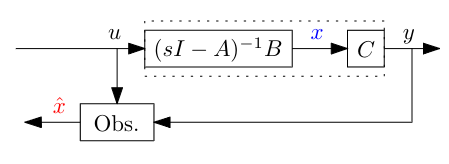
\includegraphics[width=10cm]{\imagesPath/observer.png}
    \caption{Observers}
    \label{fig:observer}
\end{figure}


\section{Memory Management}
\adef{Harvard architecture} a system that has separate memory and 
buses for code (ROM) and data (RAM).

\subsection{Read only memory (ROM)}
\begin{itemize}
    \item Store code and constants
    \item Usually difficult to write
    \item Usually Flash memory 
    \item Also exists PROM, UV-EPROM, EEPROM
    \item Pico Board has 2MB external Flash
\end{itemize}

\subsection{Random access memory (RAM)}
\begin{itemize}
    \item Stack and heap
    \item Usually SRAM or DRAM
    \item Usually Flash memory 
    \item Also exists PROM, UV-EPROM, EEPROM
    \item Pico RP2040 has 265kB on-chip SRAM divided into 6 separate modules to allow 
    6 parallel accesses.
\end{itemize}

\subsection{Read - Modify - Write}
Often we want to change just a single bit in a register. This require reading a word
modify the word using bit operations then write it back, and this is not atomic.

\begin{exampleblock}{Solution 1 - BIT-BANDING}
    \begin{tabular}{|c|c|c|c|c|c|c|c|}
        \hline
        0 & 1 & 0 & 1 & 0 & 0 & 0 & 0 \\
        \hline
    \end{tabular}

    Then if we want to access the second bit we have a alias for it 
    to a non physical memory address.
\end{exampleblock}

\begin{exampleblock}{Solution 2 - Bit Set and Clear Register}
    When set is 1 and the register is either 1 or 0 the result will be 1.
    When set is 0 the register wont change.\newline
    \begin{tabular}{ c c c c c c c c c c }
            Reg & 0 & 0 & 0 & 0 &  & 1 & 1 & 1 & 1  \\
            Set & 0 & 1 & 1 & 0 &  & 1 & 0 & 0 & 0  \\
        Result: & 0 & 1 & 1 & 0 &  & 1 & 1 & 1 & 1 
    \end{tabular}

    When CLR is 1 and the register is either 1 or 0 the result is 0.
    When CLR is 0 the register wont change.\newline
    \begin{tabular}{ c c c c c c c c c c }
            Reg & 0 & 1 & 1 & 0 &  & 1 & 1 & 1 & 1  \\
            CLR & 1 & 1 & 0 & 0 &  & 1 & 0 & 0 & 0  \\
        Result: & 0 & 0 & 1 & 0 &  & 0 & 1 & 1 & 1 
    \end{tabular}
\end{exampleblock}


\subsection{Manage memory}
At compile time (statically)
\begin{itemize}
    \item Compiler/linker creates different segments
    \begin{itemize}
        \item Code (.text)
        \item Read-only data (.rodata)
        \item Read-write data (.data)
        \item zero-initialized read-write data (.bss). 
        It is more effective to have it in a separate segment than in read-write,
        since we don't have to assign the value to each variable.
    \end{itemize}
\end{itemize}

There are also possible to do it at startup or at runtime (dynamic).
At runtime (dynamic).
\begin{itemize}
    \item Problems:
    \begin{itemize}
        \item Possibly insufficent memory during runtime
        \item Fragmentation
        \item Implementation of malloc and free can be of substantial size
    \end{itemize}
\end{itemize}

There are different modes: 
\begin{itemize}
    \item Processor mode
    \begin{itemize}
        \item Thad mode, for executing applications
        \item Handler mode, will automaticl enter this mode when there is exeption handeling and 
        then will return to thred mode whenever it is done.
    \end{itemize}
    \item Software execution modes
    \begin{itemize}
        \item Unpriviledged mode, limited access, e.g. cannot change process state.
        \item Privileged mode, has access to all resources.
    \end{itemize}
\end{itemize}

\begin{figure}[H]
    \centering
    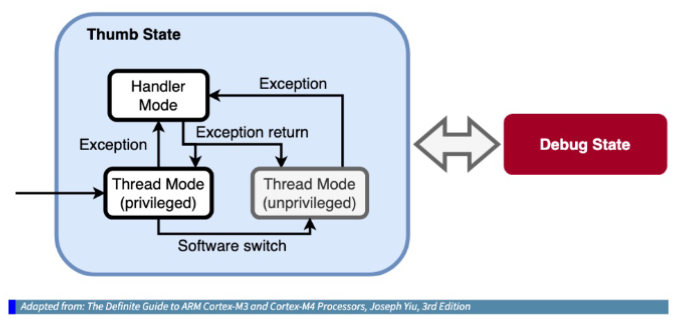
\includegraphics[width=10cm]{\imagesPath/arm_operation_modes.png}
    \caption{ARM Operation modes}
    \label{fig:arm_operation_modes}
\end{figure}

\adef{Memory protection unit} allows access rules to be set up for 
privileged access and user program access.



\section{Debugging}
From failure to fault
\begin{enumerate}
    \item Verify the failure, determine correct behavior
    \item Isolate and minimize (shrink)
    \item Eyeball the code, where could the fault be?
    \item Devise and run experiments to test your hypothesis
    \item Repeat 3 \& 4 until you understand what's wrong
    \item Create a regression test
\end{enumerate}

\subsection{Problem minimization 1: inputs}
Decrease the inputs.

\begin{itemize}
    \item Generalization of greedy binary search
    \item Basic idea 
    \begin{itemize}
        \item Divide input into chunks (initially 2)
        \item Remove a chunk, does the test still fail?
        \item If yes, continue without it
        \item If no, increase granularity (*2)
        \item Stop when curring away doesn't help anymore and number of chunks is the length of the input
    \end{itemize}
\end{itemize}

\begin{exampleblock}{Delta Debugging algorithm}
    Use the delta debugging algorithm to find the input which gives the error.
    Whenever 1, 7, and 8 is in the input there is an error.
    \begin{center}
        \begin{tabular}{ c c c c c c c c c c}
         1 & 2 & 3 & 4 & 5 & 6 & 7 & 8 & & \\ 
        \end{tabular}
    \end{center}

    Initially divide it up into two chunks.
    \begin{center}
        \begin{tabular}{ c c c c|c c c c c}
         1 & 2 & 3 & 4 & 5 & 6 & 7 & 8 \\ 
         \color{lightgray}{1} & \color{lightgray}{2} & \color{lightgray}{3} & \color{lightgray}{4} & 5 & 6 & 7 & 8 & \color{green}{\checkmark} \\ 
         1 & 2 & 3 & 4 & \color{lightgray}{5} & \color{lightgray}{6} & \color{lightgray}{7} & \color{lightgray}{8} & \color{green}{\checkmark} \\ 
        \end{tabular}
    \end{center}

    No fail increase granualarity.
    \begin{center}
        \begin{tabular}{ c c|c c|c c|c c c}
         1 & 2 & 3 & 4 & 5 & 6 & 7 & 8 \\ 
         \color{lightgray}{1} & \color{lightgray}{2} & 3 & 4 & 5 & 6 & 7 & 8 & \color{green}{\checkmark} \\ 
         1 & 2 & \color{lightgray}{3} & \color{lightgray}{4} & 5 & 6 & 7 & 8 & \color{red}{x} \\ 
        \end{tabular}
    \end{center}

    Failed, remove the chunk which did not fail.
    \begin{center}
        \begin{tabular}{ c c|c c|c c c}
         1 & 2 & 5 & 6 & 7 & 8 \\ 
         \color{lightgray}{1} & \color{lightgray}{2} & 5 & 6 & 7 & 8 & \color{green}{\checkmark} \\ 
         1 & 2 & \color{lightgray}{5} & \color{lightgray}{6} & 7 & 8 & \color{red}{x} \\ 
        \end{tabular}
    \end{center}

    Failed, remove the chunk which did not fail.
    \begin{center}
        \begin{tabular}{ c c|c c c}
         1 & 2 & 7 & 8 \\ 
         \color{lightgray}{1} & \color{lightgray}{2} & 7 & 8 & \color{green}{\checkmark} \\ 
         1 & 2 & \color{lightgray}{7} & \color{lightgray}{8} & \color{green}{\checkmark} \\ 
        \end{tabular}
    \end{center}

    No fail increase granualarity.
    \begin{center}
        \begin{tabular}{ c|c|c|c c}
         1 & 2 & 7 & 8 \\ 
         \color{lightgray}{1} & 2 & 7 & 8 & \color{green}{\checkmark} \\ 
         1 & \color{lightgray}{2} & 7 & 8 & \color{red}{x} \\ 
        \end{tabular}
    \end{center}

    Found that 1, 7, and 8 is causing the issue.
    
\end{exampleblock}


\subsection{Problem minimisation 2: Slicing}
Decrease the code.

\begin{itemize}
    \item Central concept of debugging
    \item Main idea
    \begin{itemize}
        \item Give a Program P and some occurance of variable x
        \item Remove all statements that do not affect x
        \item end up with simplified version of P' of P 
        \item P' only contains statements imports of value of x
    \end{itemize}
    \item \textit{Static backward slicing}: determine what causes the changes to the final value.
\end{itemize}


\begin{figure}[H]
    \centering
    \begin{subfigure}[b]{0.45\textwidth}
        \centering
        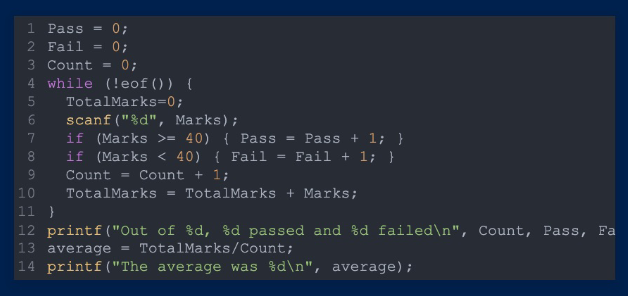
\includegraphics[width=\textwidth]{\imagesPath/cfg_code.png}
        \caption{CFG example code}
    \end{subfigure}
    \hfill
    \begin{subfigure}[b]{0.45\textwidth}
        \centering
        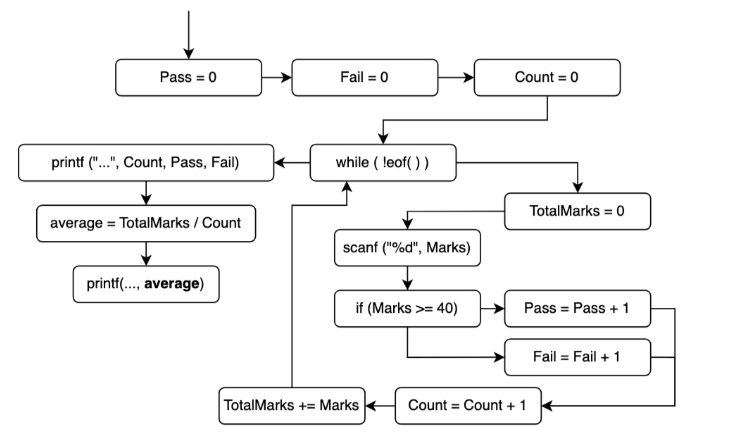
\includegraphics[width=\textwidth]{\imagesPath/cfg.png}
        \caption{CFG}
    \end{subfigure}
       \caption{Control Flow Graph (CFG)}
\end{figure}


\begin{itemize}
    \item Simple logging
    \begin{itemize}
        \item printf
        \item serial output
        \item LEDs
        \item \ldots
    \end{itemize}
    \item Logging frameworks
    \begin{itemize}
        \item log4c
        \item Zephyr logging
        \item \ldots
    \end{itemize}
    \item Using a debugger
\end{itemize}

\begin{figure}[H]
    \centering
    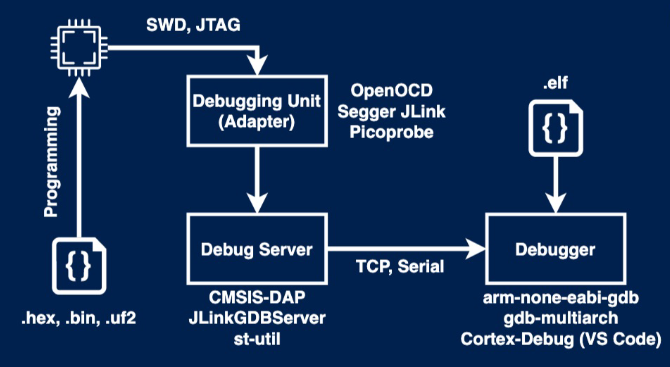
\includegraphics[width=10cm]{\imagesPath/debugging_setup.png}
    \caption{Debugging setup}
\end{figure}


\section{Optimization}
\begin{center}
    \begin{tabular}{ c c c }
     Algorithm      & WC Runtime    & AC Runtime \\ 
     Bubble-sort    & $O(n^2)$      & $O(n^2)$ \\  
     Insertion-sort & $O(n^2)$      & $O(n^2)$ \\  
     Quick-sort     & $O(n^2)$      & $O(n\log(n))$ \\  
     Merge-sort     & $O(n\log(n))$ & $O(n\log(n))$ \\  
     Tim-sort       & $O(n\log(n))$ & $O(n)$ \\  
    \end{tabular}
\end{center}
 
Different data structures has different complexity for different operations,
e.g. a array has a faster read time than a linked list.

\textit{Space - Time - Tradeoff} is when we have to choose what is more important
memory or performance. Since using little memory could worsen the performance and
focusing on performance could worsen the memory usage.
For example with a look-up table with frequently calculated values instead are precalculated 
values in a table. This cost more space but there is less computation involved.

Individual bits can be stored in different ways either.
\begin{itemize}
    \item Packed: bits are grouped together
    \item Padded: reserve whole byte/word for each bit
\end{itemize}

For instance bit fields in c where we packed a number of bits in a struct.

\textit{Alignment} is how we align data in memory. 
%Often we only can read a single word and not a single bit. However, to save space we can have multiple in the same word, which requires the data to ordered in the same way we access it. Then we can use pointer arithmatic to only get the required data.
On \textit{fully aligned} architectures, we need to have all variables aligned within a word.
On \textit{self aligned} architectures, addresses of n-byte types have to be multiples of n.
The compiler is not allowed to re-order the fields. (a word is 2 bytes).

To know what we should optimize we use a \textit{profiler} that measures the time
spent in individual functions, blocks, ...
We can also measure the performance, i.e. \textit{instrument} the code.
We can also experiment with removing or duplicate code sections.

Profilers:
\begin{itemize}
    \item Instrumentation based
    \begin{itemize}
        \item Profiler add statements to capture time at various code locations
        \item Affects overall measured time  (at times drastically)
    \end{itemize}
    \item Sampling based
    \begin{itemize}
        \item Profiler stops program periodically to record current program counter.
        So the current executed routine can be determined.
        \item This is less precis
    \end{itemize}
    \item Simulation based
    \begin{itemize}
        \item Usually quite slow
        \item Needs cycle-accurate simulator for the platform
        \item often works with simplified assumptions about the hardware
    \end{itemize}
    \item In-circuit/tracing
    \begin{itemize}
        \item Needs hardware support
        \item Often implemented by internally sampling 
    \end{itemize}
\end{itemize}

Some common thing that we can optimize to eliminate bottlenecks is:
\begin{itemize}
    \item Choose a better suited algorithm or data structure
    \item Perform low-level optimizations
    \item Optimization is related to refactoring
    \begin{itemize}
        \item We want to improve the design
        \item Modifications should not impact functionality of the systems
    \end{itemize}
\end{itemize}

\begin{itemize}
    \item Use faster instructions: Using bit operators is faster instead of for instance multiplication.
    \item Use right arithmetic data-types: Using generalized int, float, double can have significant impact on computation, memory allocations depending on microC used. Use fixed sizes that are better suited for operation/purpose. For instance, uint8\_t instead of int when doing a for loop that has a few iterations (< 256).
    \item Loop optimizations: If we have a loop that does similar operation every iteration or that iterations might not be that big, we can ask the compiler to optimize the loop by unrolling the loop for instance (loop iterations has to be known at compile time). Unrolling a loop decreases conditional checks because we are executing sequentially instead of jumping back and doing condition checks for the loop.
    \item Sub-expression elimination: the process of eliminating a process that occurs at multiple instances. For instance, when an expression is calculated at multiple places, it is maybe better to just calculate it once, save in memory and use it everywhere it is needed instead of recalculating the expression.
    \item Inlining: the process of replacing a subroutine or function call at the call site with the body of the subroutine or function being called. This eliminates call-linkage overhead and can expose significant optimization opportunities.
    \item Algebraic simplifications: Simplifying your calculations to maybe do less calculations and still get the same/similar/close-enough result.
\end{itemize}
% copied from slides and drive



\section{Testing}
Testing in form of \textit{dynamic} verifications means that we verify by running the code.
\textit{Static} verification means that we inspect the code without running it. 

\begin{itemize}
    \item Unit testing: test the low-level unit design with individual software units such as functions, classes, tasks, ...
    \item Integration testing: test the architectural design with a focus on integration/interaction between different modules/units.
    \item System testing: testing the system level specification.
    \item Acceptance testing: test the software with respect to user requirements.
    \item Orthogonal: Regression testing.
\end{itemize}

\begin{itemize}
    \item Test set: a collection of test cases for a particular unit
    \item Test suite: is a collection of test sets
\end{itemize}

\textit{Oracles} is a mechanism for determining whether a test has passed or failed.

Construction of test suites
\begin{itemize}
    \item Black box (Closed box) testing: The test are derived from the external description without any knowledge of the implementation.
    \item White box (Glass box) testing: Make test from the source code to test for instance all branches, conditions, statements, ...
\end{itemize}

Code \textit{coverage} referees to how much of the our has covered when all test has run.

\begin{itemize}
    \item Input domain modelling: All possible inputs.
    \item Input space partitioning: Partition input domain into regions.
\end{itemize}

Structural coverage 

Common notions in CFGS
\begin{itemize}
    \item Execution path: Path through CFG that start at entry point.
    \item Path condition: the condition for which the path is taken.
    \item Feasible execution path: If a path condition can be satisfied.
\end{itemize}

\begin{itemize}
    \item \textit{Statement coverage}: with all tests every node in the CFG is executed at least one.
    \item \textit{Branch coverage}: with all tests every edge in the CFG is taken at least once.
    \item \textit{Path coverage}: with all tests every possible path in the CFG is executed at least once 
    \item \textit{Decision coverage}: with at least one test where d evaluates to true and one where d evaluates to false.
    \item \textit{Condition Coverage}: for each condition c in program p evaluates as least once to true and once to false.
\end{itemize}

\begin{exampleblock}{Modified condition decision ceverage (MC/DC)}
    Let X be the condition (A \&\& (B | C))
    \begin{tabular}{|c|c|c|c|c|}
        \hline
        Test & A & B & C & X \\
        \hline
        1 & T & T & T & T \\
        \hline
        2 & T & T & F & T \\
        \hline
        3 & T & F & T & T \\
        \hline
        4 & T & F & F & F \\
        \hline
        5 & F & T & T & F \\
        \hline
        6 & F & T & F & F \\
        \hline
        7 & F & F & T & F \\
        \hline
        8 & F & F & F & F \\
        \hline
    \end{tabular}\newline

    All pairs where A changes values and the output is different but B and C is the same.\newline
    \begin{tabular}{ c }
        Test = \{1, 5\}, \{2, 6\}, \{3, 7\}
    \end{tabular}\newline

    All pairs where B changes values and the output is different but A and C is the same.\newline
    \begin{tabular}{ c }
        Test = \{2, 4\}
    \end{tabular}\newline

    All pairs where C changes values and the output is different but A and B is the same.\newline
    \begin{tabular}{ c }
        Test = \{3, 4\}
    \end{tabular}\newline

    To have tests that cover at least one pair of each boolean variable:\newline
    \begin{tabular}{ c }
        Test = \{2, 3, 4, 6\}
    \end{tabular}
    %https://www.youtube.com/watch?v=bwtALQVx86w
\end{exampleblock}

\textit{Regression testing}: test which runs when new features or when we refactor code to prevent 
the introduction of new bugs.


\section{Verification}
\adef{Program verifier} takes a program specification and program code
and verifies it, i.e. proves the programs correctness.
If it finns a counter examples it proves that the code is incorrect.
It can also be inconclusive were no conclusion can be drown.

\adef{Abstract interpretation} techniques based on fixed-point computation.
Widely used by compilers. Use specification to create a mathematical structure for the prof.

\adef{Model checking} a technics based on (systematic) state-space exploration.

\adef{Heuristic Bug finders} focus on implicit specifications.


\subsection{Transition systems}
\adef{transition systems} is a concept used to study the computation.
A program can be converted into a number of possible state the variables can be 
in. A state space is noted as $S$ and the initial state $I$ were $I\subseteq S$, 
and transitions $\rightarrow \subseteq S \times S$.

The goal is to identify if there is a set of $Err \subseteq S$ error states.
The system is safe if there is no path $s_0 \rightarrow s_1 \rightarrow \ldots \rightarrow s_n$
with $s_0\in I$ and $s_n\in Err$.

\begin{figure}[H]
    \centering
    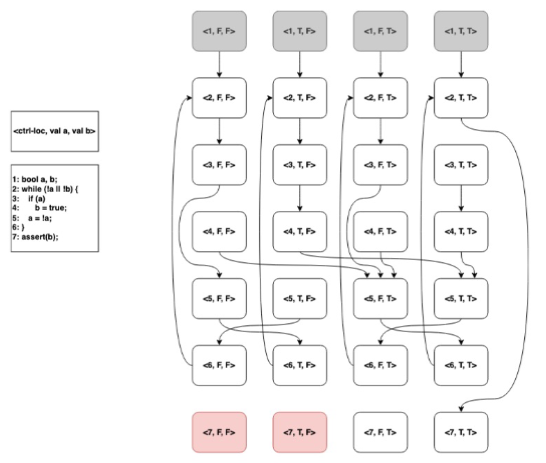
\includegraphics[width=10cm]{\imagesPath/transition_systems.png}
    \caption{Transition Systems}
\end{figure}

\adef{Explicit state model checking}: explicitly construct graph ($S, I, \rightarrow$) and check 
reachability of error states. There are a few languages that does support it like java with 
\textit{Java Path Finder}.


\subsection{Deductive Verification}
Deductive software verification aims at formally verifying that all possible behaviors of a given program satisfy formally defined, possibly complex properties, where the verification process is based on some form of logical inference, i.e., “deduction”.

\adef{Hoare logic} has the goal to provide a formal system for reasoning about program correctness.
\begin{exampleblock}{Hoare logic example}
    \begin{lstlisting}[language=c]
        /*
            PRE: a > 0
            POST: ret > 0
        */
        int f(int a) {
            /* { a > -1 } => is implied by PRE */
            int x = a;
            /* { x > -1 } */
            x = 2 * x;
            /* { x > -2 } */
            x = x + 2;
            /* { x > 0 } */
            return x;
        }
    \end{lstlisting}
    Start at the end and work your way up.
\end{exampleblock}
